\section{Nivel II: análisis estadístico de tolerancias}
\label{sec:nivel2}

Este nivel optativo estudia cómo se dispersa la respuesta del filtro \emph{construido} (componentes de la \cref{tab:bom}, TL072) cuando los
componentes varían dentro de su tolerancia. Siguiendo la guía, se definen las distribuciones (a), se ejecutan en LTspice \nNRun{} corridas distintas por
escenario, documentando cómo se generan las muestras (b), se obtienen las distribuciones de los parámetros y el porcentaje de cumplimiento (c), se
comparan con la predicción por sensibilidad lineal de la \cref{sec:sensibilidad} (d) y se repite el análisis con tolerancias menores (e). Todo el
procesamiento está en el notebook~05.

\subsection{Distribuciones y escenarios}
Cada componente se modela como una variable aleatoria \textbf{uniforme e independiente} en $[x_0(1-t),\,x_0(1+t)]$, con $x_0$ el valor nominal y $t$
la tolerancia. Como solo se conoce el intervalo que garantiza el fabricante, es la hipótesis más conservadora. Las resistencias armadas con dos
en serie se sortean \emph{por separado}, como ocurre en el circuito real, de modo que varían nueve elementos por corrida; la resistencia del generador
($R_s = \qty{50}{\ohm}$) se mantiene fija. La \cref{tab:mc_escenarios} resume los cuatro escenarios: E1 es el ejemplo de la guía, E2 corresponde a los
componentes del prototipo (resistencias de \qty{1}{\percent} y capacitores código~K) y E3--E4 repiten el análisis con capacitores más precisos.

\begin{table}[H]
  \centering\small
  \caption{Escenarios del análisis de tolerancias.}
  \label{tab:mc_escenarios}
  \tabres{tab_mc_escenarios}
\end{table}

Un filtro \emph{cumple} si satisface la plantilla original (no la función de diseño): atenuación máxima en la banda de paso
$A_{p,\max} = \max_{f \le f_p} G - \min_{f \le f_p} G \le \qty{1}{\decibel}$ y atenuación en el borde de rechazo
$A(f_s) = \max_{f \le f_p} G - G(f_s) \ge \qty{24}{\decibel}$, con $G = 20\log_{10}|V_6/V_{in}|$. Además de estas dos magnitudes se registran la
atenuación en \qty{1}{\kilo\hertz}, la frecuencia de \qty{-3}{\decibel} y los parámetros del circuito $f_r$, $f_0$ y $Q$.

\subsection{Generación de las muestras en LTspice}
La función \texttt{mc(x,t)} de LTspice devuelve un número con distribución uniforme entre $x(1-t)$ y $x(1+t)$. Se escribe directamente en el valor
de cada elemento, por ejemplo \texttt{C1 4 6 \{mc(47n,tolC)\}}, de modo que cada elemento recibe su propio sorteo, y la directiva
\texttt{.step param run 1 500 1} repite el análisis AC \nNRun{} veces, volviendo a sortear todos los valores en cada paso. El parámetro
\texttt{run} solo numera las corridas. Las tolerancias se fijan con \texttt{.param tolR=... tolC=...}, y un netlist por escenario
(\texttt{ltspice/filtro\_TL072\_mc\_E1.cir} a \texttt{\_E4.cir}) usa el modelo de TI del TL072 con $\pm\qty{12}{\volt}$ y un barrido de
\qty{10}{\hertz} a \qty{100}{\kilo\hertz} con 50 puntos por década. El listado del escenario E2 es:

\VerbatimInput[fontsize=\footnotesize,frame=single,framesep=2mm]{\ltsdir/filtro_TL072_mc_E2.cir}

Para que el muestreo sea verificable, el netlist incluye dos \emph{sondas} desacopladas del filtro: resistencias de valor \texttt{\{mc(1,tolR)\}} y
\texttt{\{mc(1,tolC)\}} alimentadas con \qty{1}{\ampere}, cuya tensión es numéricamente el número sorteado en cada corrida y queda registrada en el
\texttt{.log}. Como en la \cref{sec:ltspice}, antes de correr LTspice el netlist se resolvió con el solver nodal propio, con cada \texttt{mc()}
reemplazado por su valor central y AO ideales: coincide con la transferencia del circuito con un error relativo máximo de \num{\nErrNet}.

\subsubsection{Verificación del muestreo}
Las cuatro corridas de LTspice (versión 24.1.10) completaron los \nNRun{} pasos de cada escenario y \num{\nVerifDistintasMin} de cada \num{\nNRun}
resultados de $A(\qty{1}{\kilo\hertz})$ son distintos entre sí: \textbf{las corridas son efectivamente distintas}. Los números sorteados por las sondas
cubren el intervalo declarado y su distribución es compatible con la uniforme (prueba de Kolmogorov--Smirnov, $p \ge \num{\nKSsondaMin}$;
\cref{fig:mc_muestreo}).

\begin{figure}[H]
  \centering
  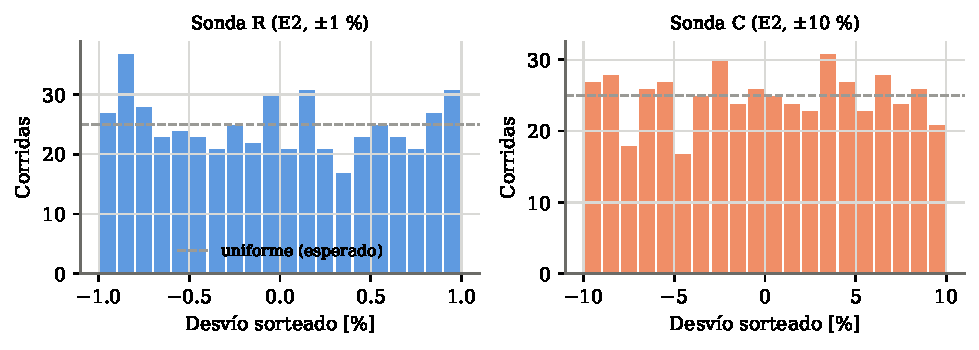
\includegraphics[width=0.85\textwidth]{fig_mc_muestreo}
  \caption{Números sorteados por las sondas en las \nNRun{} corridas del escenario E2, expresados como desvío respecto del nominal. La línea
  punteada es la altura esperada para una distribución uniforme.}
  \label{fig:mc_muestreo}
\end{figure}

Las sondas mostraron además que \textbf{LTspice usa siempre la misma secuencia de números aleatorios}: en los cuatro escenarios, y en ejecuciones
distintas, los desvíos normalizados $u = (x/x_0 - 1)/t$ son idénticos. Cada escenario es una muestra válida, pero los cuatro comparten los mismos
sorteos, escalados por su tolerancia; en estadística esto se conoce como \emph{números aleatorios comunes} y tiene una ventaja: las diferencias entre
escenarios se deben solo a las tolerancias y no al azar del muestreo. La contrapartida es que cualquier particularidad de la muestra aparece en los
cuatro escenarios a la vez.

Para examinar el generador se armó el netlist \texttt{filtro\_mc\_sondas.cir}: los mismos nueve elementos, con los mismos nombres y en el mismo orden
que el del escenario E2, pero aislados del filtro y excitados de modo que su valor quede registrado (las resistencias con \qty{1}{\ampere}, los
capacitores con \qty{1}{\volt} a \qty{1}{\kilo\hertz}). Sus sondas coinciden exactamente con las del Monte Carlo E2, de modo que este netlist
\textbf{recupera el valor de los nueve componentes en cada una de las \nNRun{} corridas}. Con esos valores se verificó lo siguiente.
\begin{itemize}
  \item \textbf{Contraste corrida por corrida} (\cref{fig:mc_por_corrida}): con los mismos componentes, la transferencia exacta con AO ideales y
        LTspice con el TL072 difieren como máximo en \qty{\nPcMaxAp}{\decibel} en $A_{p,\max}$ y \qty{\nPcMaxGunok}{\decibel} en
        $A(\qty{1}{\kilo\hertz})$. En $f_0$ y $Q$ las diferencias son prácticamente constantes, de \qty{\nPcMedFo}{\percent} y
        \qty{\nPcMedQ}{\percent}: es el efecto del GBW finito del TL072 previsto en la \cref{sec:sensibilidad}. En $f_{-3\,\text{dB}}$ la diferencia
        media es de \qty{\nPcMedFtres}{\percent}, a la que también contribuye la interpolación de \texttt{.meas} sobre la grilla de 50 puntos por
        década. Solo \nPcVeredictos{} de los \num{2000} circuitos simulados recibe un veredicto de cumplimiento distinto, un caso de E1 que está
        justo en el límite de \qty{1}{\decibel}.
  \item \textbf{Distribución y correlaciones de los sorteos}: los once sorteos de cada corrida son compatibles con la distribución uniforme. Entre los
        55 pares posibles, \nParesFuera{} superan el límite del \qty{95}{\percent} para variables independientes ($|r| < \num{\nRLimite}$), lo
        esperable por azar (unos 3). Pero el par $C_1$--$C_2$ tiene una correlación muestral de $r = \num{\nRCunoCdos}$, poco probable por azar.
        Como $\ln f_0 \propto -(\ln C_1 + \ln C_2)/2$ y $\ln Q \propto (\ln C_1 - \ln C_2)/2$, esa correlación agranda la dispersión de $f_0$ y
        achica la de $Q$, y explica por qué en esta muestra $\sigma(f_0)$ resulta un \qty{10}{\percent} mayor y $\sigma(Q)$ un \qty{7}{\percent}
        menor que lo esperado (\cref{tab:mc_dispersion}).
  \item \textbf{Secuencia larga}: para decidir si esa correlación es un defecto del generador o una particularidad de la muestra se corrió el mismo
        netlist con \num{5000} pasos (\texttt{filtro\_mc\_sondas\_5000.cir}). Sus primeras 500 corridas son idénticas a las anteriores. En las
        \num{5000}, la correlación $C_1$--$C_2$ es $r = \num{\nRCunoCdosLargo}$, dentro del límite de $\pm\num{\nRLimiteLargo}$, y solo
        \nParesFueraLargo{} de los 55 pares lo superan. En los nueve bloques de 500 corridas que siguen al primero, $r(C_1, C_2)$ varía entre
        \num{\nRBloqMin} y \num{\nRBloqMax}. La correlación de \num{\nRBloqUno} es entonces una \textbf{particularidad de las primeras 500 corridas
        de la secuencia fija de LTspice}, no un defecto del generador.
\end{itemize}
En consecuencia, las 500 corridas de LTspice son una muestra legítima pero particular. Para estimar la población se usa la referencia de Python
con \num{\nMPy} muestras, y la comparación con LTspice se hace teniendo en cuenta su error muestral.

\begin{figure}[H]
  \centering
  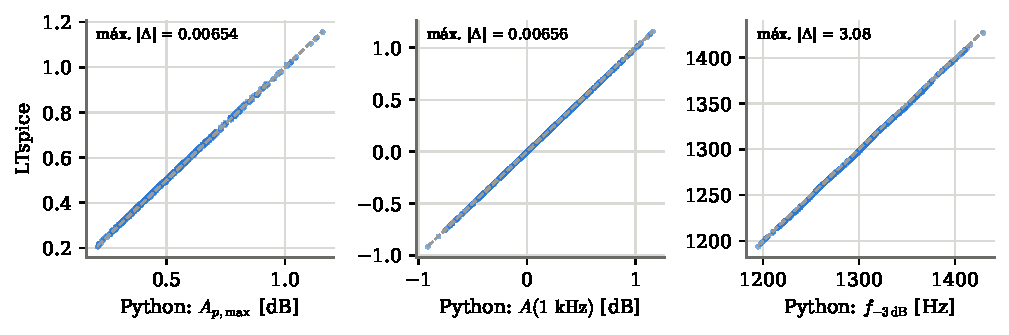
\includegraphics[width=\textwidth]{fig_mc_por_corrida}
  \caption{Contraste corrida por corrida del escenario E2: cada punto es un circuito del Monte Carlo, evaluado en LTspice (TL072) y en Python
  (transferencia exacta, AO ideales) con los mismos valores de componentes, recuperados con \texttt{filtro\_mc\_sondas.cir}.}
  \label{fig:mc_por_corrida}
\end{figure}

\subsection{Referencia en Python y predicción lineal}
Como referencia independiente de LTspice, el mismo experimento se repite en Python con \num{\nMPy} muestras por escenario, sobre la transferencia
exacta del circuito con AO ideales, en la misma grilla de frecuencias que LTspice y con las mismas definiciones de $A_{p,\max}$ y $A(f_s)$.

La predicción lineal usa las sensibilidades de la \cref{sec:sensibilidad}, ahora respecto de los nueve elementos. Una variación relativa
$\delta_x$ de cada elemento produce $\Delta P \approx \sum_x S^P_x\,\delta_x$ y, para variables uniformes independientes
($\sigma_{\delta_x} = t_x/\sqrt{3}$),
\begin{equation}
  \sigma_P \approx \sqrt{\sum_x \left(S^P_x\right)^2 \frac{t_x^2}{3}} .
  \label{eq:sigma_lineal}
\end{equation}
$A_{p,\max}$ es el máximo de la atenuación sobre la banda de paso y no es una función lineal de los componentes. En el filtro nominal ese máximo está
en el valle interior del rizado, cerca de \qty{530}{\hertz}, pero cuando $f_0$ o $f_r$ bajan pasa al borde de \qty{1}{\kilo\hertz}. Por eso, para
predecir su distribución se usa un \emph{Monte Carlo linealizado}: con las mismas muestras, la ganancia en cada frecuencia de la grilla se aproxima por
$G_0(f) + \sum_x S^{G}_x(f)\,\delta_x$ y luego se aplican las mismas definiciones. Así la no linealidad del máximo se conserva, pero cada ganancia se
evalúa con la aproximación de primer orden.

\subsection{Resultados}
La \cref{fig:mc_curvas} muestra las \nNRun{} respuestas del escenario E2, junto con la nominal y el prototipo medido; la
\cref{fig:mc_histogramas} muestra las distribuciones de los parámetros y la \cref{fig:mc_rendimiento} y la \cref{tab:mc_rendimiento} resumen el
porcentaje de cumplimiento.

\begin{figure}[H]
  \centering
  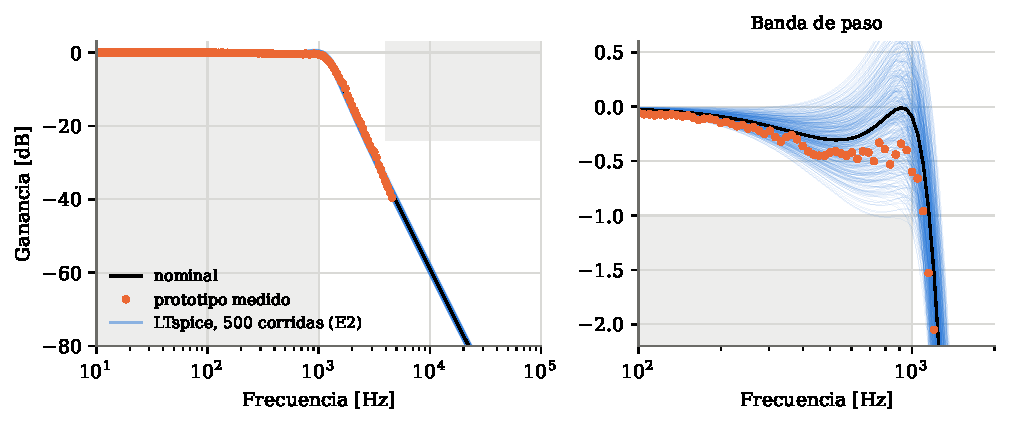
\includegraphics[width=\textwidth]{fig_mc_curvas}
  \caption{Las \nNRun{} respuestas del escenario E2 (LTspice, TL072), la respuesta nominal y el prototipo medido (\cref{sec:mediciones}). Las
  zonas grises son las regiones prohibidas por la plantilla. A la derecha, detalle de la banda de paso.}
  \label{fig:mc_curvas}
\end{figure}

\begin{figure}[H]
  \centering
  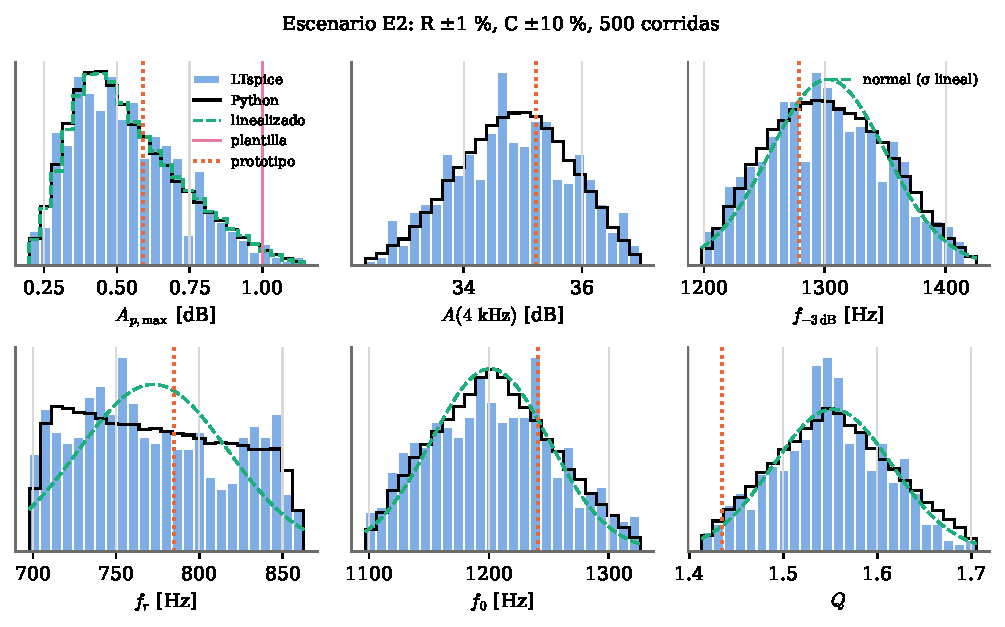
\includegraphics[width=\textwidth]{fig_mc_histogramas}
  \caption{Distribuciones del escenario E2: LTspice (\nNRun{} corridas, barras), Python (\num{\nMPy} muestras, escalones) y predicción lineal (para
  $A_{p,\max}$, el Monte Carlo linealizado; para $f_{-3\,\text{dB}}$, $f_r$, $f_0$ y $Q$, una normal con la $\sigma$ de la
  \cref{eq:sigma_lineal}). La línea vertical continua es el límite de la plantilla y la punteada, el prototipo medido.}
  \label{fig:mc_histogramas}
\end{figure}

\begin{figure}[H]
  \centering
  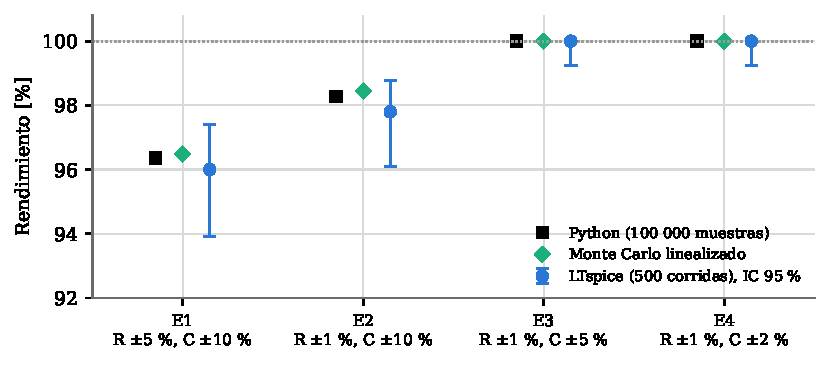
\includegraphics[width=0.85\textwidth]{fig_mc_rendimiento}
  \caption{Porcentaje de filtros que cumplen la plantilla en cada escenario. Las barras de LTspice son el intervalo de confianza del
  \qty{95}{\percent} (Wilson) para \nNRun{} corridas.}
  \label{fig:mc_rendimiento}
\end{figure}

\begin{table}[H]
  \centering\small
  \caption{Rendimiento (porcentaje de filtros que cumplen la plantilla) y percentil 95 de $A_{p,\max}$.}
  \label{tab:mc_rendimiento}
  \tabres{tab_mc_rendimiento}
\end{table}

\paragraph{Cumplimiento.} Con los componentes del prototipo (E2), LTspice da un rendimiento del \qty{\nRendLtDos}{\percent} (intervalo del
\qty{95}{\percent}: \numrange{\nRendLtInfDos}{\nRendLtSupDos}), compatible con el \qty{\nRendPyDos}{\percent} de Python y con el
\qty{\vRendDiez}{\percent} estimado en la etapa de diseño (\cref{sec:margen}). En E1 (resistencias de \qty{5}{\percent}) baja al \qty{\nRendLtUno}{\percent}.
En todos los casos la condición que falla es la del rizado: la atenuación a \qty{4}{\kilo\hertz} nunca baja de \qty{\nAcuatroMinLtUno}{\decibel},
contra \qty{24}{\decibel} exigidos, y la atenuación mínima entre \qty{4}{\kilo\hertz} y \qty{100}{\kilo\hertz} coincide en cada corrida con la de
\qty{4}{\kilo\hertz}: el TL072 no deja pasar señal en alta frecuencia en ninguna corrida. Sin el margen de diseño de la \cref{sec:margen}, el
rendimiento sería de apenas un \qty{\vRendSinMargen}{\percent}, aun con capacitores de \qty{\pm 5}{\percent}.

\paragraph{Distribuciones.} $A_{p,\max}$ tiene una distribución asimétrica, con cola hacia valores altos: es el máximo de la atenuación sobre la
banda de paso y, cuando $f_0$ o $f_r$ bajan, el máximo salta del valle interior del rizado al borde de \qty{1}{\kilo\hertz}. $f_r$ depende casi solo
de $C_0$ (\qty{\pm 10}{\percent}) y de $R_0$ (\qty{\pm 1}{\percent}), por lo que su distribución es prácticamente uniforme. $f_0$ y $Q$ combinan
dos capacitores y tienen una forma triangular; $A(\qty{4}{\kilo\hertz})$ y $f_{-3\,\text{dB}}$ combinan más elementos y se acercan a una normal.
En los cuatro escenarios, la prueba de Kolmogorov--Smirnov entre LTspice y Python no rechaza la igualdad de distribuciones para $A_{p,\max}$ ni para
$A(\qty{1}{\kilo\hertz})$ ($p \ge \num{0.4}$). Solo en E4, donde la dispersión es más chica, rechaza para $f_{-3\,\text{dB}}$ ($p = \num{0.001}$) y, en el límite, para $Q$
($p = \num{0.04}$): los corrimientos sistemáticos del modelo con TL072 medidos en el contraste corrida por corrida
(\qty{\nPcMedFtres}{\percent} y \qty{\nPcMedQ}{\percent}) ya no son despreciables frente a una dispersión de menos del \qty{1}{\percent}.

\paragraph{Comparación con la sensibilidad lineal (d).} La \cref{tab:mc_dispersion} compara las desviaciones estándar del escenario E2. La predicción
lineal coincide con el Monte Carlo de Python dentro del \qty{1}{\percent} en todos los parámetros: con tolerancias de hasta \qty{10}{\percent}, el
filtro se comporta de forma prácticamente lineal y la \cref{eq:sigma_lineal} basta para estimar la dispersión. El Monte Carlo linealizado reproduce
también el rendimiento (\qty{\nRendLinDos}{\percent} frente a \qty{\nRendPyDos}{\percent}) y el percentil 95 de $A_{p,\max}$
(\cref{tab:mc_rendimiento}). Las diferencias entre la columna de Python con \num{\nMPy} muestras y LTspice se deben a la muestra particular
analizada en la subsección anterior: evaluada en Python con los mismos 500 juegos de componentes, la dispersión coincide con la de LTspice. La
forma de la distribución, en cambio, no siempre es normal (\cref{fig:mc_histogramas}): para $f_r$, la $\sigma$ lineal es correcta, pero la
distribución es uniforme y sus colas son más cortas que las de una normal.

\begin{table}[H]
  \centering\small
  \caption{Desviación estándar de los parámetros en el escenario E2 (R $\pm\qty{1}{\percent}$, C $\pm\qty{10}{\percent}$): predicción lineal
  (\cref{eq:sigma_lineal}), Monte Carlo de Python con \num{\nMPy} muestras y con los mismos 500 juegos de componentes de LTspice, y LTspice.
  Frecuencias y $Q$ en porcentaje del valor nominal.}
  \label{tab:mc_dispersion}
  \tabres{tab_mc_dispersion_E2}
\end{table}

\paragraph{Tolerancias menores (e).} Con capacitores de \qty{\pm 5}{\percent} (E3) o \qty{\pm 2}{\percent} (E4), los 500 circuitos de LTspice y los
\num{\nMPy} de Python cumplen la plantilla. El percentil 95 de $A_{p,\max}$ baja a \qty{\nApNoventaLtTres}{\decibel} y
\qty{\nApNoventaLtCuatro}{\decibel}, respectivamente, y la dispersión de cada parámetro escala casi proporcionalmente a la tolerancia de los
capacitores, que dominan el error (la de $A(\qty{1}{\kilo\hertz})$ pasa de \qty{\nSigAunokLtDos}{\decibel} en E2 a \qty{\nSigAunokLtTres}{\decibel}
en E3 y \qty{\nSigAunokLtCuatro}{\decibel} en E4). Para un diseño de producción, pasar a capacitores código~J eliminaría prácticamente las fallas
sin cambiar la topología. Bajar la tolerancia de las resistencias, en cambio, aporta poco: de E1 a E2, con los mismos capacitores, el rendimiento
mejora apenas dos puntos.

\paragraph{El prototipo dentro de la distribución.} Con los parámetros medidos (\cref{sec:mediciones}), el prototipo es un caso
típico del escenario E2 en casi todo: un \qty{\nUbicAp}{\percent} de los circuitos simulados tiene un $A_{p,\max}$ mayor que el medido, un
\qty{\nUbicFr}{\percent} se aparta más que él en $f_r$ y un \qty{\nUbicFo}{\percent} tiene una $f_0$ más alta. El parámetro menos típico es $Q$,
\qty{7.6}{\percent} por debajo del nominal: solo un \qty{\nUbicQ}{\percent} de los circuitos simulados tiene un $Q$ más bajo. Es coherente con la
estimación de los capacitores, con $C_1$ en el límite inferior de su tolerancia y $C_2$ por encima del nominal. Aun así, el prototipo cumple la
plantilla con margen, que es justamente lo que el margen de diseño buscaba asegurar.

\paragraph{Conclusión del Nivel II.} El análisis estadístico confirma el diseño: con los componentes disponibles, cerca del \qty{98}{\percent} de los
filtros construidos cumpliría la plantilla, y la causa de las fallas restantes (el rizado, por el desvío de los capacitores) está identificada. Las
tres vías de cálculo independientes coinciden dentro del error estadístico: LTspice con el modelo del fabricante, la transferencia exacta en Python y
la predicción lineal por sensibilidades. El procedimiento quedó documentado de forma verificable: corridas distintas, distribución de los sorteos
comprobada y valores de cada corrida recuperados y contrastados uno a uno.
